\section*{Discussion}
The present study shows that ConvMixer \cite{trockman2022patchesneed} is a strong and parameter-efficient candidate for Vietnamese speech command classification, with representative performance of 97.14\% test accuracy, macro-F1 0.9716, and weighted-F1 0.9714 at 719,117 parameters ($\sim$0.72M). In the revised protocol, we frame this result as empirical evidence to be interpreted together with controlled cross-model comparisons and multi-seed statistics, rather than as an isolated superiority claim.

\subsection*{ConvMixer Efficiency Profile}

From the controlled benchmark in Table~\ref{tab:controlled_model_comparison}, ConvMixer-256/8 provides a strong efficiency-oriented operating point. Compared with ResNet-18 (11.17M parameters), ConvMixer uses only 0.72M parameters while maintaining competitive recognition quality (97.14\% accuracy vs. 98.46\%). It also outperforms AST (tiny) by a wide margin on accuracy/F1 while requiring lower training time than larger convolutional baselines such as EfficientNet.

This profile supports the practical positioning of ConvMixer as a compact architecture that preserves high task performance with substantially lower model size, which is especially relevant for memory-constrained and edge-oriented deployments.

\subsection*{Controlled Comparison and Statistical Reliability}

To directly address reviewer concerns on fairness and stability, we incorporated a controlled comparison protocol (Section Results, Table~\ref{tab:controlled_model_comparison}) using ConvMixer-256/8, ResNet-18, MobileNetV2, EfficientNet, and AST (tiny configuration) under aligned preprocessing, feature extraction, split policy, and training budget. In addition, each model is evaluated with five seeds (42--46), and final performance is reported as mean$\pm$std. Under the current logged benchmark results, ResNet-18 leads on raw accuracy/F1, while ConvMixer provides the most compact high-performing profile and a favorable quality-to-size trade-off. This revision shifts interpretation from single-run outcomes to statistically grounded model behavior and enables clearer model-level trade-off analysis.

\subsection*{Practical Applications and Deployment Feasibility}
From an application perspective, the proposed system targets command-driven voice interfaces in smart homes and IoT environments, where always-on recognition must be lightweight, responsive, and sufficiently robust under background noise. Typical scenarios include local control of lighting, fan, TV, and curtain systems, as well as privacy-preserving on-device wake-command modules that avoid continuous cloud transmission.

Regarding deployment feasibility, the controlled comparison indicates that ConvMixer-256/8 offers a favorable balance between recognition quality and resource usage, especially when contrasted with heavier baselines. This makes ConvMixer a practical candidate for CPU-oriented and low-power edge platforms, provided that implementation-level optimization (e.g., kernel scheduling and quantization-aware deployment) is further applied. Therefore, the main practical value of this work is not only classification performance, but also the reproducible efficiency profile needed for embedded integration.

\subsection*{Language Scope and Generalization Considerations}
The current benchmark is built on Vietnamese commands, so direct claims to multilingual generalization remain out of scope. Nonetheless, the modeling principle is language-agnostic at the feature and architecture levels (Mel-spectrogram input and patch-based convolutional mixing). In practice, transfer to other languages is expected to depend on phonetic inventory differences, pronunciation variability, recording conditions, and command-set design.

Accordingly, we treat cross-language transfer as a structured future evaluation problem rather than an implicit assumption. A rigorous follow-up should include multilingual or cross-lingual protocols (train-on-language A, test-on-language B, and mixed-language training) to quantify robustness and calibration behavior under language shift.

\subsection*{Extended Evaluation on the UrbanSound8K Dataset}

Beyond the experiments conducted on the self-collected Vietnamese speech command dataset, we further evaluated the proposed
approach on the widely used UrbanSound8K dataset~\cite{Salamon2014UrbanSound} as an auxiliary experiment to assess the generalization capability of the ConvMixer architecture in a broader audio classification context. Prior studies on UrbanSound8K have reported strong performance using CNN-based architectures such as CNN14 and the PANN family, as well as lightweight transformer-inspired models~\cite{9229505,hershey2017cnnarchitectureslargescaleaudio}. In this experiment, the ConvMixer-256/8 model was retrained following the same preprocessing pipeline and training configuration described previously. As illustrated in Figure~\ref{fig:train_val_curves_us8k}, the model demonstrates rapid convergence and stable validation performance despite the substantial acoustic differences between environmental sounds and short spoken command signals.

Quantitatively, the model achieved 96\% accuracy and a macro F1-score of approximately 0.96 on the official test split of UrbanSound8K, showing performance comparable to several contemporary approaches reported in the literature, including representative CNN-based and MLP-based architectures. These reference models provide competitive baselines for environmental sound classification, making the comparison particularly meaningful when assessing the generalization capability of ConvMixer. These results underscore that even without relying on complex self-attention mechanisms, ConvMixer remains competitive due to its efficient patch-based representation and the separation of spatial--channel mixing through depthwise and pointwise convolutions.

To provide deeper insight into the model’s per-class performance, Figure~\ref{fig:conf_matrix_us8k} presents the
confusion matrix for all ten UrbanSound8K categories. Several classes such as \textit{air\_conditioner},
\textit{engine\_idling}, and \textit{gun\_shot} exhibit near-perfect precision and recall, while minor misclassifications
primarily occur among acoustically similar classes such as \textit{street\_music} and \textit{children\_playing}. Overall,
the confusion matrix highlights the robustness of ConvMixer across diverse and complex acoustic patterns, reinforcing
its applicability beyond the domain of speech command recognition.

\begin{figure}[htbp]
    \centering
    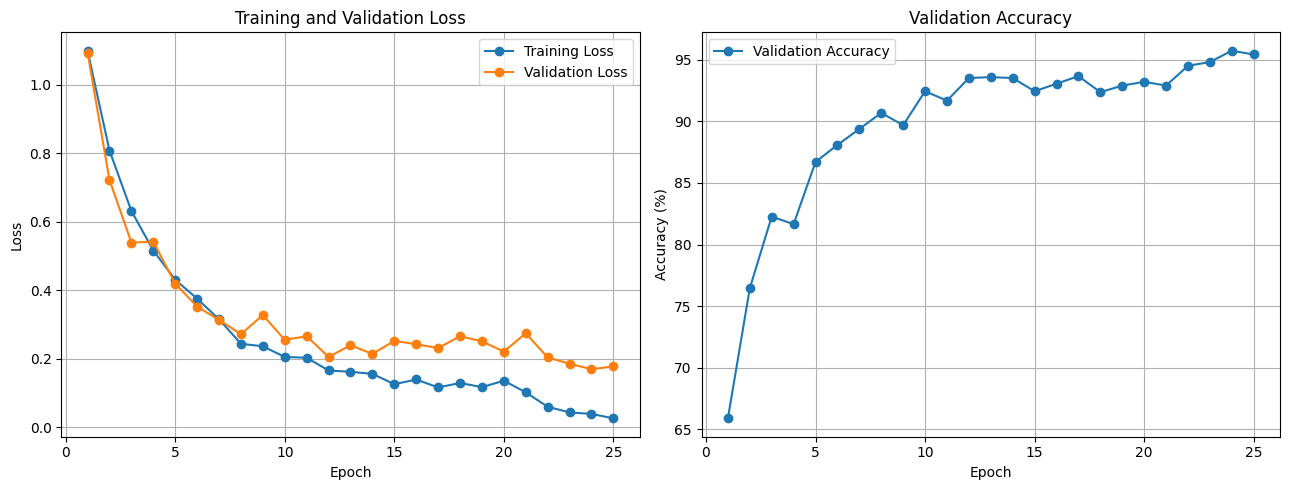
\includegraphics[width=0.9\linewidth]{imgs/train_val_loss_acc_2.png}
    \caption{Training and validation curves (training loss, validation loss, and validation accuracy) of the ConvMixer-256/8 model on the UrbanSound8K dataset.}
    \label{fig:train_val_curves_us8k}
\end{figure}

\begin{figure}[htbp]
    \centering
    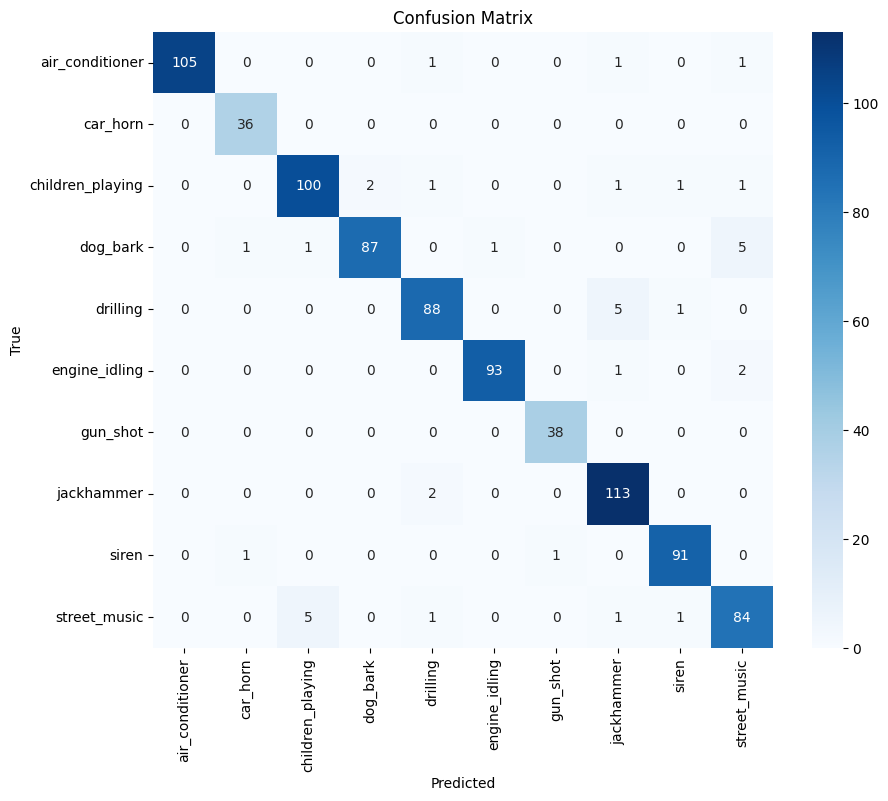
\includegraphics[width=0.75\linewidth]{imgs/cfs_matrix_2.png}
    \caption{Confusion matrix of the ConvMixer-256/8 model on the UrbanSound8K test set.}
    \label{fig:conf_matrix_us8k}
\end{figure}


\subsection*{Analysis of Architectural Performance}
The competitive behavior of ConvMixer \cite{trockman2022patchesneed} can be interpreted from its architectural design, which combines patch processing with convolutional inductive bias. First, treating the Mel-spectrogram \cite{Stevens1937MelScale} as a 2D input and dividing it into patches using a 7x7 embedding layer causes downsampling to occur early, increasing the effective receptive field and facilitating long-range spatial modeling. Second, ConvMixer performs spatial and channel mixing via Depthwise Convolution (9x9) and Pointwise Convolution (1x1), respectively, enabling efficient capture of time--frequency textures and inter-channel interactions. This structure, together with residual connections and isotropic blocks, helps maintain favorable optimization behavior on modest-scale datasets.

\subsection*{Observations on Misclassification Errors}
Despite the high overall test accuracy, the detailed analysis of the classification report revealed minor classification errors concentrated in commands with close acoustic or semantic relationships. Two classes, including the crucial \textit{unknown} class, achieved perfect F1-scores of 1.00 (\textit{unknown}, \textit{dong\_rem}). The most notable discrepancies occurred between the contrasting commands \textit{bat\_quat} (turn on fan) and \textit{tat\_quat} (turn off fan), with F1 scores of 0.9444 and 0.9429, respectively. The command \textit{bat\_quat} shows precision/recall of 0.9189/0.9714, while \textit{tat\_quat} records 0.9429/0.9429, indicating bidirectional confusion in acoustically similar fan-related commands. Additional mild recall drops are also visible for \textit{bat\_tv} and \textit{mo\_rem} (both 0.9412 recall). These residual errors are consistent with subtle phonetic overlap and time-frequency similarity in short utterances, even after robust preprocessing (VAD \cite{WebRTCVAD}, denoising, two-stage high-energy extraction).

\subsection*{Limitations of the Current Study}
While demonstrating strong efficacy, the current investigation is subject to several limitations that warrant future research. Firstly, the dataset scale is relatively small, consisting of 4,460 samples across 13 classes of Vietnamese speech commands. Although ConvMixer demonstrated high data efficiency on this scale, its performance and generalization capabilities should be further validated on larger and more diverse datasets (e.g., AudioSet \cite{Gemmeke2017AudioSet}). Secondly, although lightweight CNN and transformer baselines (ResNet-18 and AST with tiny configuration) are incorporated in the controlled benchmark, broader transformer variants and larger pretraining-based models remain to be evaluated under the same protocol. Thirdly, while a unified preprocessing ablation protocol and reporting table are now defined, further extensions with additional acoustic conditions can strengthen causal interpretation of front-end contributions. Lastly, although parameter efficiency is high ($\sim$0.72M), architectural documents suggest that ConvMixer may exhibit lower throughput than highly optimized alternatives such as DeiT \cite{Touvron2020DeiT}, likely due to large depthwise kernels and patch settings. In addition, the present configuration space remains limited; broader hyperparameter sweeps over depth, width, and kernel size may provide additional gains.

\subsection*{Potential Future Improvements}

Based on these findings, several promising directions for future research are identified. Firstly, given the success of ViT-based models \cite{dosovitskiy2020image} in leveraging large-scale pretraining, exploring transfer learning or self-supervised pretraining regimes on extensive audio datasets such as AudioSet \cite{Gemmeke2017AudioSet} could significantly enhance ConvMixer's robustness and generalization. 

Secondly, although ConvMixer emphasizes convolutional operations \cite{trockman2022patchesneed}, integrating it with lightweight self-attention modules offers a promising avenue to improve long-range feature modeling while maintaining computational efficiency. We plan to investigate hybrid ConvMixer–attention architectures to combine the benefits of local inductive bias and global contextual reasoning.

Thirdly, to facilitate deployment in embedded and edge-AI applications, low-level optimization of the large-kernel depthwise convolutions should be pursued to further improve inference throughput. 

Finally, beyond speech command recognition, ConvMixer can be extended to non-speech audio domains such as environmental sound classification, acoustic scene analysis, or emotional speech recognition. Expanding the application scope will help validate the model’s scalability and strengthen its contribution to the broader field of lightweight audio understanding.
